% Experiment 2 — SCS-CN runoff (separate from Week 5 Lab 2)
% Folder: Experiment-reports/Experiment2_SCSCN_Runoff/
% Build: pdflatex Experiment2_SCSCN_Runoff_Report.tex (twice)
%
\documentclass[11pt,a4paper]{article}

\usepackage[margin=2.5cm]{geometry}
\usepackage{graphicx}
\usepackage{booktabs}
\usepackage{amsmath}
\usepackage{xurl}
\usepackage{hyperref}
\usepackage{parskip}
\usepackage{enumitem}
\usepackage{fvextra}
\usepackage[most]{tcolorbox}

\newcommand{\studentname}{Mahmudul Hasan}
\newcommand{\studentid}{4125999049}
\newcommand{\reportdate}{May 22, 2026}

\makeatletter
\g@addto@macro\UrlBreaks{\do\ }
\makeatother

\newcommand{\LabCodeRoot}{files}

\newcommand{\filebox}[2]{%
\begin{tcolorbox}[
  enhanced,
  colback=gray!6,
  colframe=black!55,
  title={#1},
  fonttitle=\bfseries\ttfamily\footnotesize,
  arc=1.5mm,
  boxrule=0.7pt,
  breakable,
  width=\linewidth,
  before skip=0.8em,
  after skip=0.8em,
]
\VerbatimInput[fontsize=\footnotesize,breaklines=true,breakanywhere=true]{\LabCodeRoot/#2}
\end{tcolorbox}%
}

\title{Experiment Report: Specialized Experiment 2\\Hydrological Modeling --- SCS-CN Runoff}
\author{\studentname \quad (Student ID: \studentid)}
\date{\reportdate}

\begin{document}
\maketitle

\begin{abstract}
SCS-CN direct runoff with $S=25400/\mathrm{CN}-254$~mm, $I_a=0.2S$, and $Q=(P-I_a)^2/(P-I_a+S)$ when $P>I_a$. Hand verification at $P=50$~mm, $\mathrm{CN}=80$: $Q=13.80$~mm. Includes CN sensitivity curves, rainfall--runoff plots, physical validation matrix, and 20 pytest boundary cases with $Q\le P$ enforced.
\end{abstract}

\begin{tcolorbox}[
  colback=blue!4,
  colframe=blue!55!black,
  title=\textbf{Key Findings (Executive Summary)},
  fonttitle=\bfseries,
  arc=2mm,
]
\begin{tabular}{@{}ll@{}}
\textbf{Finding} & \textbf{Result} \\
\hline
Hand check ($P=50$, $\mathrm{CN}=80$) & $Q = 13.80$~mm \\
Automated tests & 20 passed \\
Physical rule $Q \le P$ & Verified on grid \\
CN sensitivity at $P=50$~mm & 1.40 -- 50.00~mm \\
Validation CLI & PASS \\
\end{tabular}
\end{tcolorbox}

\section{Introduction}
The SCS-CN method estimates rainfall excess (direct runoff) from total storm depth $P$ and a land-surface curve number $\mathrm{CN}$. Retention $S = 25400/\mathrm{CN} - 254$~mm and initial abstraction $I_a = 0.2\,S$ define the threshold below which no runoff occurs. This experiment translates the governing equations into tested Python code and explores sensitivity of $Q$ to $\mathrm{CN}$.

\section{Objectives}
\begin{itemize}[noitemsep]
  \item Implement \texttt{calculate\_runoff(P, CN)} with physical boundaries.
  \item Test edge cases ($P=0$, $P < I_a$, $P = I_a$, $\mathrm{CN}=100$).
  \item Perform sensitivity analysis and visualize $Q$ vs $P$ and $Q$ vs $\mathrm{CN}$.
  \item Validate $Q \le P$ and higher $\mathrm{CN}$ $\rightarrow$ higher $Q$ at fixed $P$.
  \item Document AI-assisted development in \texttt{prompt\_log.md}.
\end{itemize}

\subsection{Role in the Integrated Smart Water Pipeline}
Experiment~2 is the \textbf{rainfall-to-runoff transformation stage} in the suite workflow. Given storm depth $P$ (mm) from monitoring or design scenarios, it:
\begin{itemize}[noitemsep]
  \item converts rainfall to direct runoff $Q$ using the USDA SCS-CN method with enforced physical bounds ($Q \le P$);
  \item quantifies parameter uncertainty via a curve-number band CN $\in [75,85]$ at fixed $P$;
  \item provides runoff depths and sensitivity tables that represent plausible inflow inputs for Experiment~3 (reservoir dispatch) and inform flood-risk context for Experiment~4.
\end{itemize}
This stage links meteorological forcing to operational water-volume estimates used in storage management.

\section{Methods}

\subsection{Governing equations}
\begin{align}
S &= \frac{25400}{\mathrm{CN}} - 254 \quad \text{(mm)} \\
I_a &= 0.2\,S \\
Q &= 0 \quad \text{if } P \le I_a \\
Q &= \frac{(P - I_a)^2}{P - I_a + S} \quad \text{otherwise}, \quad Q \le P
\end{align}

\subsection{Implementation}
\texttt{scscn\_runoff.py} provides \texttt{calculate\_runoff()}, \texttt{calculate\_S()}, and \texttt{calculate\_Ia()}. Invalid inputs raise \texttt{ValueError} ($P < 0$ or $\mathrm{CN} \notin (0,100]$).

\subsection{Testing}
\texttt{test\_scscn.py} --- pytest suite covering guide cases and parametrized checks that $Q \le P$.

\subsection{Sensitivity analysis}
\texttt{sensitivity\_analysis.py} --- at $P=50$~mm, $\mathrm{CN} \in \{60,70,80,90,95,100\}$; rainfall--runoff curves for $P \in [0,120]$~mm with $I_a$ marked for $\mathrm{CN}=80$.

\subsection{Workflow}
Figure~\ref{fig:arch} shows module separation: core formula, pytest validation, sensitivity plots, and \texttt{validate\_reference.py} for reproducible hand calculations.

\begin{figure}[htbp]
  \centering
  
\includegraphics[width=0.72\linewidth,keepaspectratio]{screenshots/architecture.png}
  \caption{Code structure: runoff core $\rightarrow$ validate $\rightarrow$ test $\rightarrow$ sensitivity plots.}
  \label{fig:arch}
\end{figure}

\section{Results}

\subsection{Performance summary}
\begin{table}[htbp]
  \centering
  \caption{Experiment 2 metrics.}
  \label{tab:metrics}
  \begin{tabular}{@{}ll@{}}
    \toprule
    Metric & Result \\
    \midrule
    Pytest & 20 passed \\
    Validation CLI & \texttt{validate\_reference.py} \\
    Hand check $P=50$, $\mathrm{CN}=80$ & $Q = 13.80$~mm \\
    $\mathrm{CN}$ sensitivity at $P=50$ & 1.40 -- 50.00~mm \\
    Physical rule $Q \le P$ & Verified on grid \\
    Main figure & \texttt{runoff\_comparison.png} \\
    \bottomrule
  \end{tabular}
\end{table}

\subsection{Hand calculation verification}
For $P=50$~mm, $\mathrm{CN}=80$:
\begin{align*}
S &= 25400/80 - 254 = 63.5~\text{mm}, \quad I_a = 12.7~\text{mm} \\
Q &= (50-12.7)^2 / (50-12.7+63.5) = 13.8~\text{mm}
\end{align*}
Code: \texttt{calculate\_runoff(50, 80)} $= 13.8025$~mm (within 0.1~mm).

\begin{figure}[htbp]
  \centering
  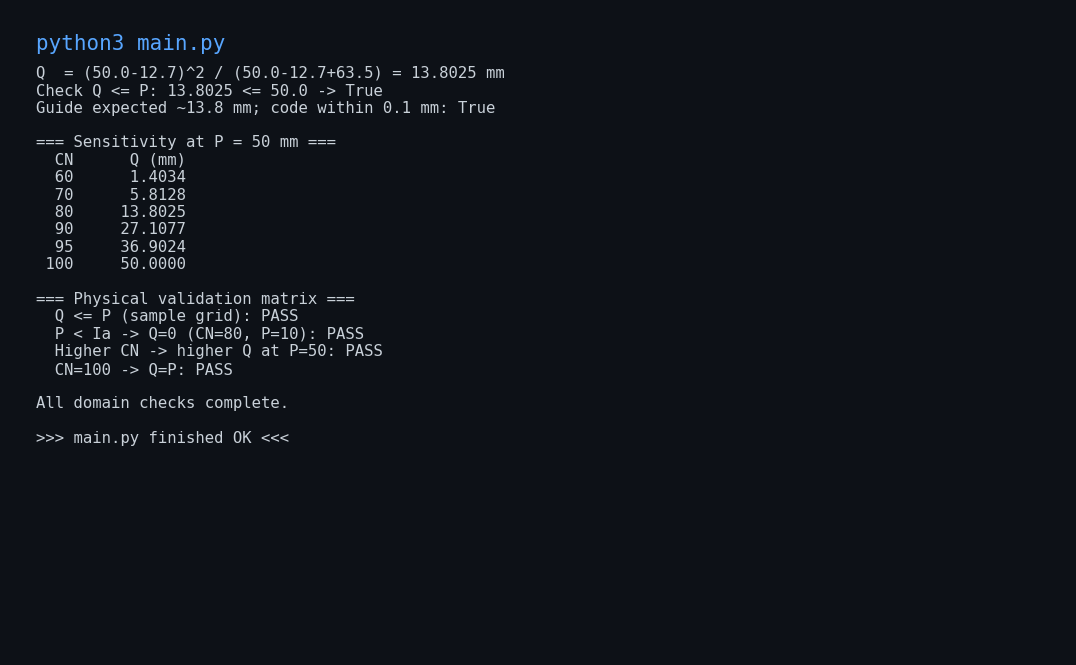
\includegraphics[width=\linewidth,height=0.42\textheight,keepaspectratio]{screenshots/experiment2_main.png}
  \caption{Pipeline run: \texttt{python3 main.py} (hand calculation, sensitivity table, physical checks).}
  \label{fig:main}
\end{figure}

\begin{figure}[htbp]
  \centering
  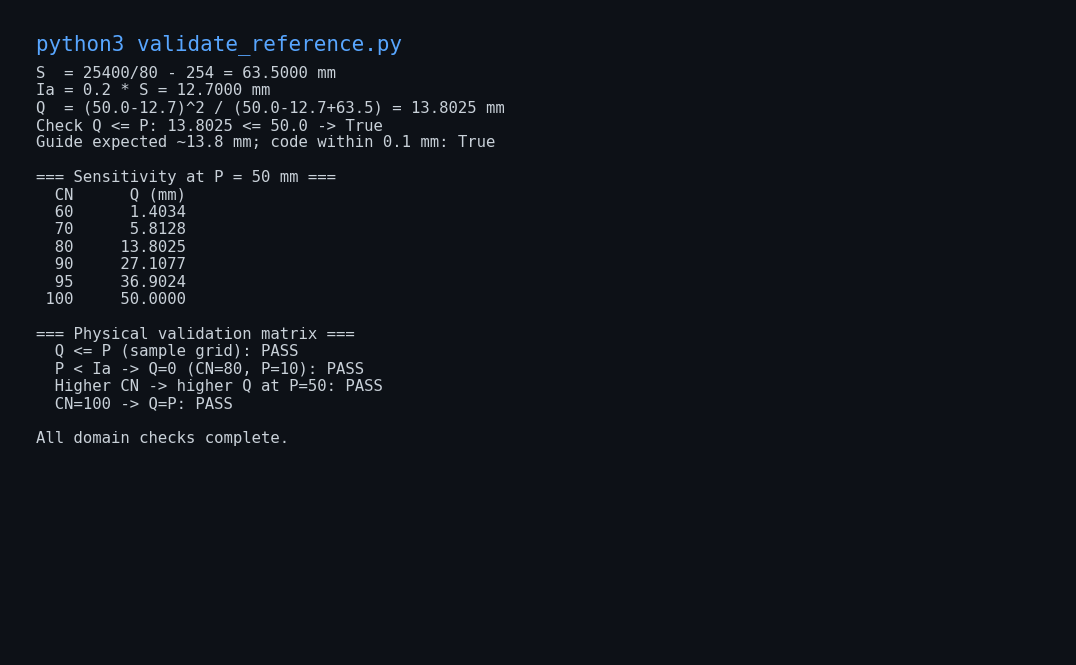
\includegraphics[width=\linewidth,height=0.42\textheight,keepaspectratio]{screenshots/experiment2_validation.png}
  \caption{CLI validation: step-by-step hand calculation and physical checks (\texttt{validate\_reference.py}).}
  \label{fig:validation}
\end{figure}

\subsection{Curve number context}
\begin{table}[htbp]
  \centering
  \caption{Typical CN ranges (experiment guide).}
  \label{tab:landuse}
  \small
  \begin{tabular}{@{}ll@{}}
    \toprule
    Land use / condition & Typical CN \\
    \midrule
    Woods, good & 60--70 \\
    Pasture, fair & 75--85 \\
    Cultivated & 80--90 \\
    Urban residential & 75--95 \\
    Paved & 95--100 \\
    \bottomrule
  \end{tabular}
\end{table}

\subsection{Automated tests}
\begin{table}[htbp]
  \centering
  \caption{Boundary test summary (pytest).}
  \label{tab:tests}
  \begin{tabular}{@{}ll@{}}
    \toprule
    Case & Expected \\
    \midrule
    $P = 0$ & $Q = 0$ \\
    $P < I_a$ & $Q = 0$ \\
    $P = I_a$ & $Q = 0$ \\
    $P = 50$, $\mathrm{CN} = 80$ & $Q \approx 13.8$~mm \\
    $\mathrm{CN} = 100$ & $Q = P$ (impervious) \\
    All tested pairs & $Q \le P$ \\
    \bottomrule
  \end{tabular}
\end{table}

\begin{figure}[htbp]
  \centering
  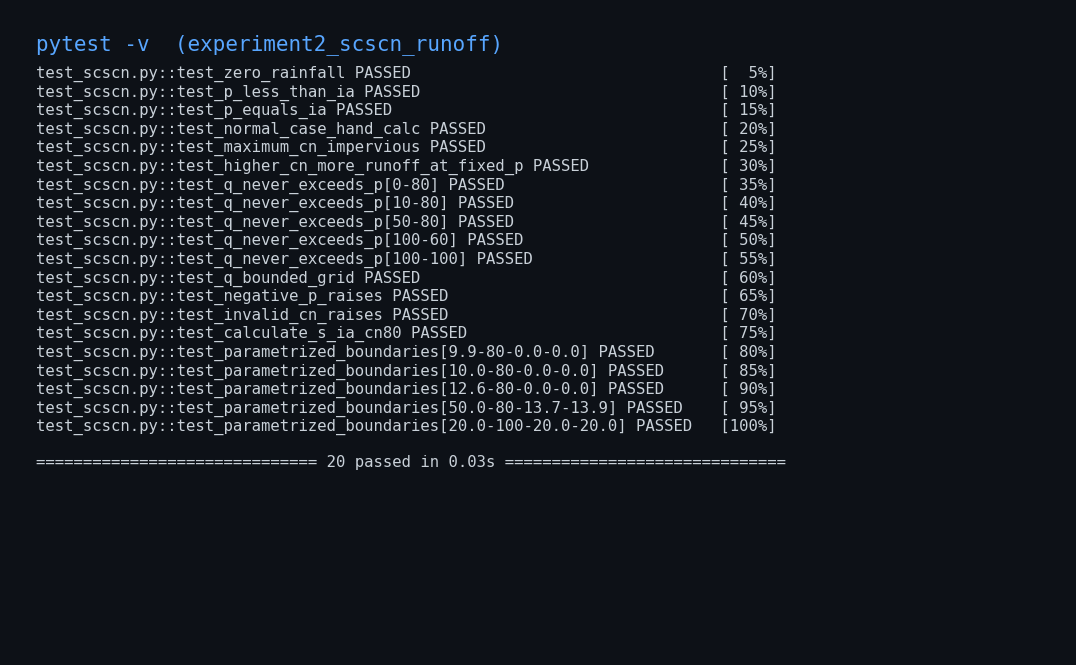
\includegraphics[width=\linewidth,height=0.38\textheight,keepaspectratio]{screenshots/experiment2_pytest.png}
  \caption{Automated test run: 20 passed (\texttt{pytest -v}), including parametrized boundaries.}
  \label{fig:pytest}
\end{figure}

\subsection{Physical validation matrix}
\begin{table}[htbp]
  \centering
  \caption{Domain constraints verified.}
  \label{tab:physics}
  \begin{tabular}{@{}ll@{}}
    \toprule
    Check & Result \\
    \midrule
    $Q \le P$ (grid sample) & PASS \\
    $P < I_a \Rightarrow Q=0$ & PASS \\
    Higher CN $\Rightarrow$ higher $Q$ at $P=50$ & PASS \\
    $\mathrm{CN}=100 \Rightarrow Q=P$ & PASS \\
    Hand calc $P=50$, $\mathrm{CN}=80$ & $\approx 13.8$~mm \\
    \bottomrule
  \end{tabular}
\end{table}

\subsection{Sensitivity at $P = 50$ mm}
\begin{table}[htbp]
  \centering
  \caption{Runoff vs curve number at fixed rainfall.}
  \label{tab:cn50}
  \begin{tabular}{@{}rr@{}}
    \toprule
    CN & $Q$ (mm) \\
    \midrule
    60 & 1.40 \\
    70 & 5.81 \\
    80 & 13.80 \\
    90 & 27.11 \\
    95 & 36.90 \\
    100 & 50.00 \\
    \bottomrule
  \end{tabular}
\end{table}

\begin{figure}[htbp]
  \centering
  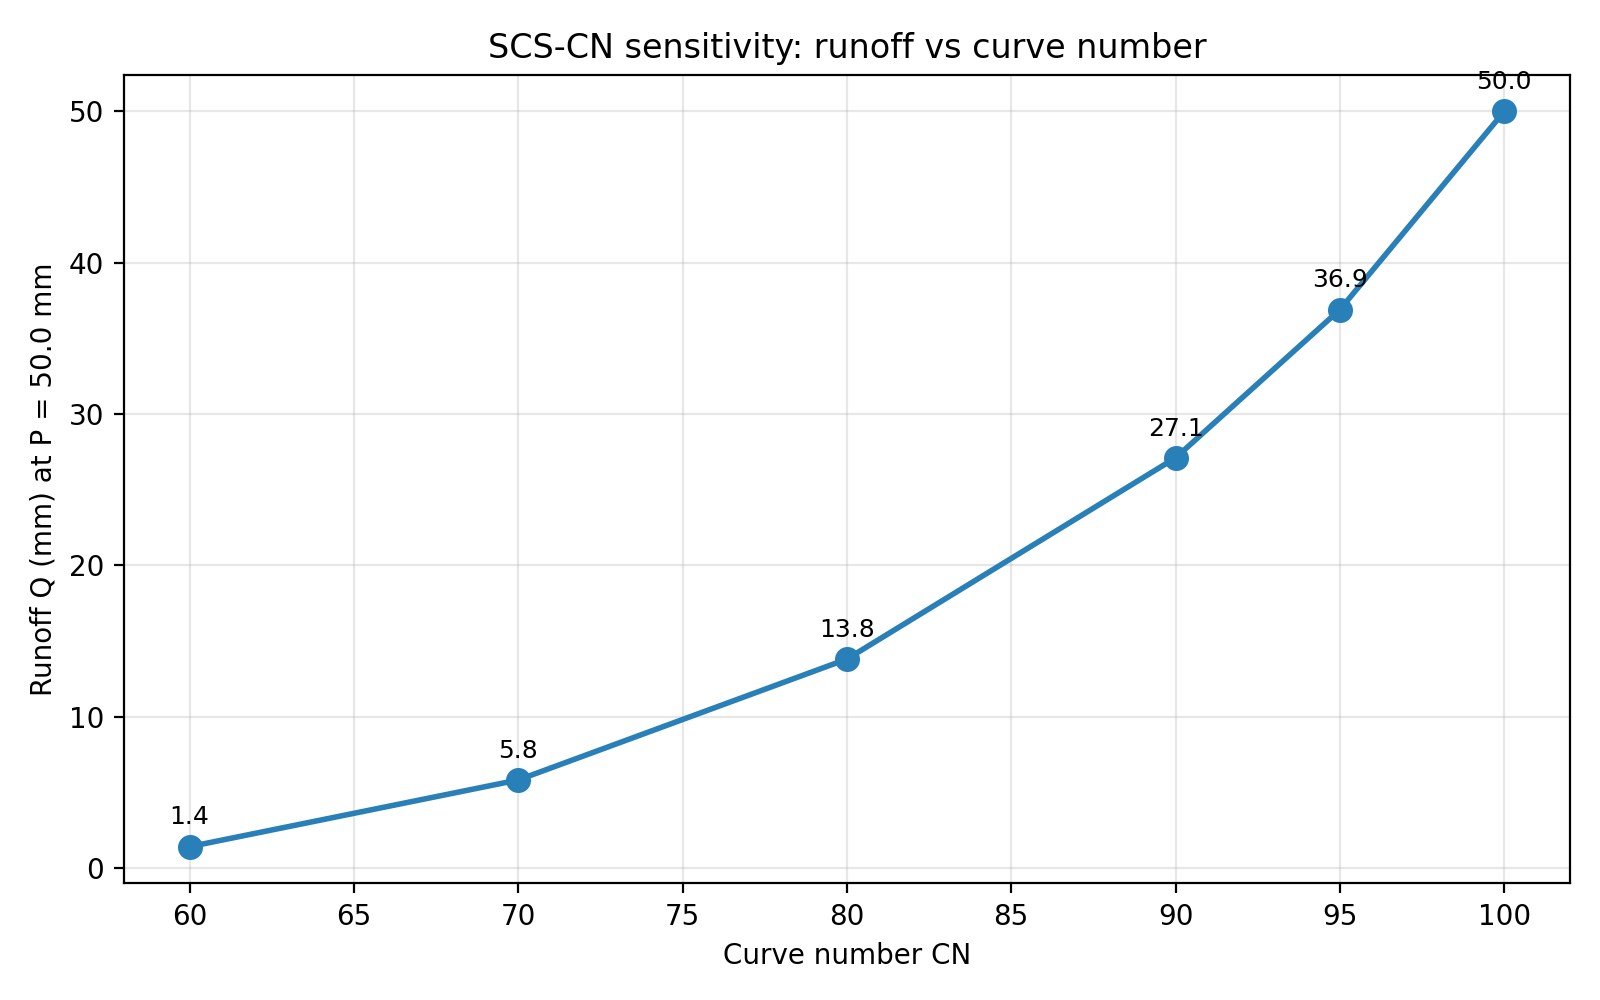
\includegraphics[width=\linewidth,height=0.48\textheight,keepaspectratio]{screenshots/cn_sensitivity.png}
  \caption{Sensitivity: runoff $Q$ vs curve number at $P = 50$~mm.}
  \label{fig:cn}
\end{figure}

\subsection{Rainfall vs runoff}
\begin{figure}[htbp]
  \centering
  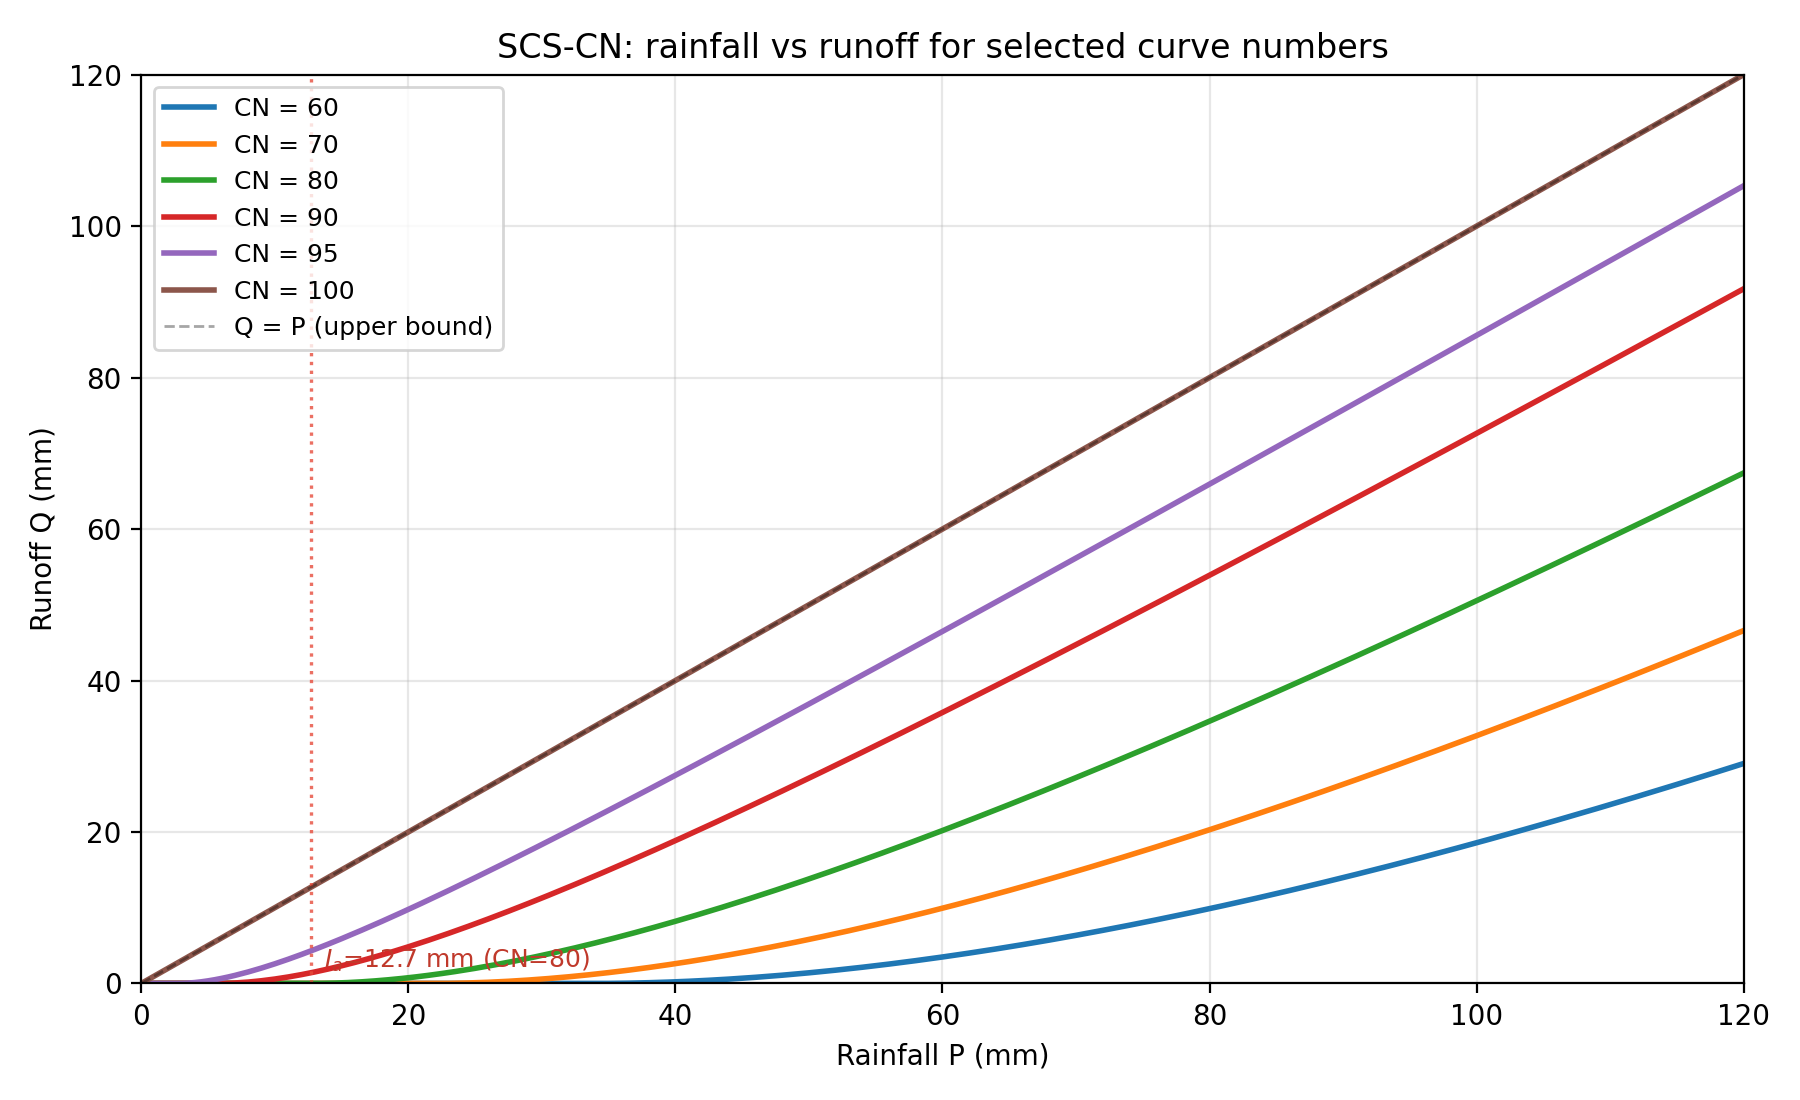
\includegraphics[width=\linewidth,height=0.52\textheight,keepaspectratio]{screenshots/runoff_comparison.png}
  \caption{Rainfall $P$ vs runoff $Q$ for $\mathrm{CN} = 60, 70, 80, 90, 95, 100$ (dashed: $Q=P$ bound).}
  \label{fig:runoff}
\end{figure}

Higher $\mathrm{CN}$ shifts curves upward: more impervious land produces more direct runoff for the same storm depth. At $\mathrm{CN}=100$, runoff equals rainfall for $P>0$.

\section{Discussion}
Results match standard SCS-CN behaviour: no runoff when rainfall is absorbed by initial abstraction, increasing runoff fraction as $\mathrm{CN}$ rises, and $Q$ bounded by $P$. The experiment guide reference ($13.8$~mm at $P=50$, $\mathrm{CN}=80$) agrees with the implementation.

\section{Lessons learned}
\begin{itemize}[noitemsep]
  \item Edge cases ($P \le I_a$) must be tested before trusting AI-generated formulas.
  \item Parametrized tests for $Q \le P$ catch cap logic errors quickly.
  \item Sensitivity plots make the $\mathrm{CN}$--runoff relationship visible for report discussion.
  \item Keeping Experiment~2 in its own folder avoids confusion with Week~5 Lab~2 naming (\texttt{src/runoff.py}).
  \item Physical validation (hand calc + monotonic $\mathrm{CN}$) is stronger evidence than code alone.
  \item A dedicated validation CLI mirrors what instructors expect in a lab notebook, not only unit tests.
\end{itemize}

\section{AI-Augmented Software Engineering}
\label{sec:ai-eng}

\subsection{Swiss Cheese Model --- layered verification}
\begin{table}[htbp]
  \centering
  \caption{Verification layers (Experiment 2).}
  \label{tab:swiss2}
  \begin{tabular}{@{}ll@{}}
    \toprule
    Layer & Result \\
    \midrule
    AI formula draft vs NRCS & Correct $S=25400/\mathrm{CN}-254$ \\
    Unit tests & 20 passed \\
    Physical constraints & $Q\ge 0$, $Q\le P$, CN bounds \\
    Edge cases & $P=0$, $P\le I_a$, CN=100 \\
    Hand validation CLI & PASS ($Q=13.80$~mm at $P=50$, CN=80) \\
    \bottomrule
  \end{tabular}
\end{table}

\subsection{Jagged Frontier --- AI mistake caught}
\textbf{AI output:} Common hallucination uses $25400\times\mathrm{CN}-254$ or forgets the $Q=0$ branch when $P\le I_a$.

\textbf{Detection:} Hand calculation and pytest normal case locked to 13.80~mm; parametrized $Q\le P$ grid.

\textbf{Human correction:} Inclusive $P\le I_a$ comparison; \texttt{min(Q,P)} cap; \texttt{validate\_reference.py} for reproducible audit.

\subsection{Tool evaluation (summary)}
Cursor Agent implemented and tested the module; ChatGPT/Gemini used for rubric alignment. Tests remain the source of truth.

\section{Reproducibility}
\label{sec:repro2}

\textbf{Environment:} Python 3.8+; \texttt{requirements.txt}.

\begin{verbatim}
pip install -r requirements.txt
pytest -v
python3 sensitivity_analysis.py
python3 validate_reference.py
python3 generate_report_figures.py
\end{verbatim}

\textbf{AI protocol:} \texttt{AGENTS.md} + \texttt{prompt\_log.md}.

\section{Conclusion}
Experiment~2 deliverables are complete with strengthened evidence: \texttt{scscn\_runoff.py}, \texttt{test\_scscn.py} (20 tests), \texttt{sensitivity\_analysis.py}, \texttt{validate\_reference.py}, \texttt{runoff\_comparison.png}, \texttt{cn\_sensitivity.png}, and \texttt{prompt\_log.md}. Figures~\ref{fig:arch}--\ref{fig:runoff} document workflow, validation, tests, and hydrologic sensitivity.

\appendix

\section{Implementation: \texttt{scscn\_runoff.py}}
\filebox{\texttt{scscn\_runoff.py}}{scscn_runoff.py}

\section{Tests: \texttt{test\_scscn.py}}
\filebox{\texttt{test\_scscn.py}}{test_scscn.py}

\section{Sensitivity: \texttt{sensitivity\_analysis.py}}
\filebox{\texttt{sensitivity\_analysis.py}}{sensitivity_analysis.py}

\section{Prompt log: \texttt{prompt\_log.md}}
\filebox{\texttt{prompt\_log.md}}{prompt_log.md}

\end{document}
